\documentclass[main]{subfiles}

\begin{document}

% \resetcounters

\section{}

\begin{definition}
	Пусть $ X $, $ A $ --- топологические пространства и $ A \ssq X $. Тогда
	\begin{itemize}
		\item если непрерывное отображение $ h \colon X \to A $ таково, что $ h_A = \Id_A $,
			то его называют \emph{ретракцией топологического пространства $ X $ на подпространство $ A $};
		\item если для подпространства $ A $ существует ретракция $ X $ на $ A $, то это подпространстов называется
			\emph{ретрактом топологического пространства $ X $}.
	\end{itemize}
\end{definition}

\begin{theorem}[Бр\'{а}уэра]
	Для любой непрерывной функции $ f \colon \D^2 \to \D^2 $ существует такая точка $ x \in \D^2 $, что $ f(x) = x $.
\end{theorem}

\begin{proof}
	Докажем методом от противного. Пусть существует такео непрерывное отображение $ f \colon \D^2 \to \D^2 $,
	что для любой точки $ x \in \D^2 $ верное $ f(x) \neq x $.

	Определим отображение $ h  \colon \D^2 \to \S^1 $ следующим образом: для каждой точки $ x \in \D^2 $ проведем
	открытый луч от точки $ f(x) $ к точке $ x $ и положим $ h(x) $ --- пересечение этого луча с окружностью.
	Так как $ f(x) \neq x $, то отображение корректно определено. Заметим, что $ h_{\S^1} = \Id_{\S^1} $.
	Очевидно, отображение $ h $ непрерывно (неформально, при непрерывном изменении точки $ x $ точка $ f(x) $
	меняется непрерывно, а значит, и открытый луч тоже).

	\begin{figure}[H]
		\centering 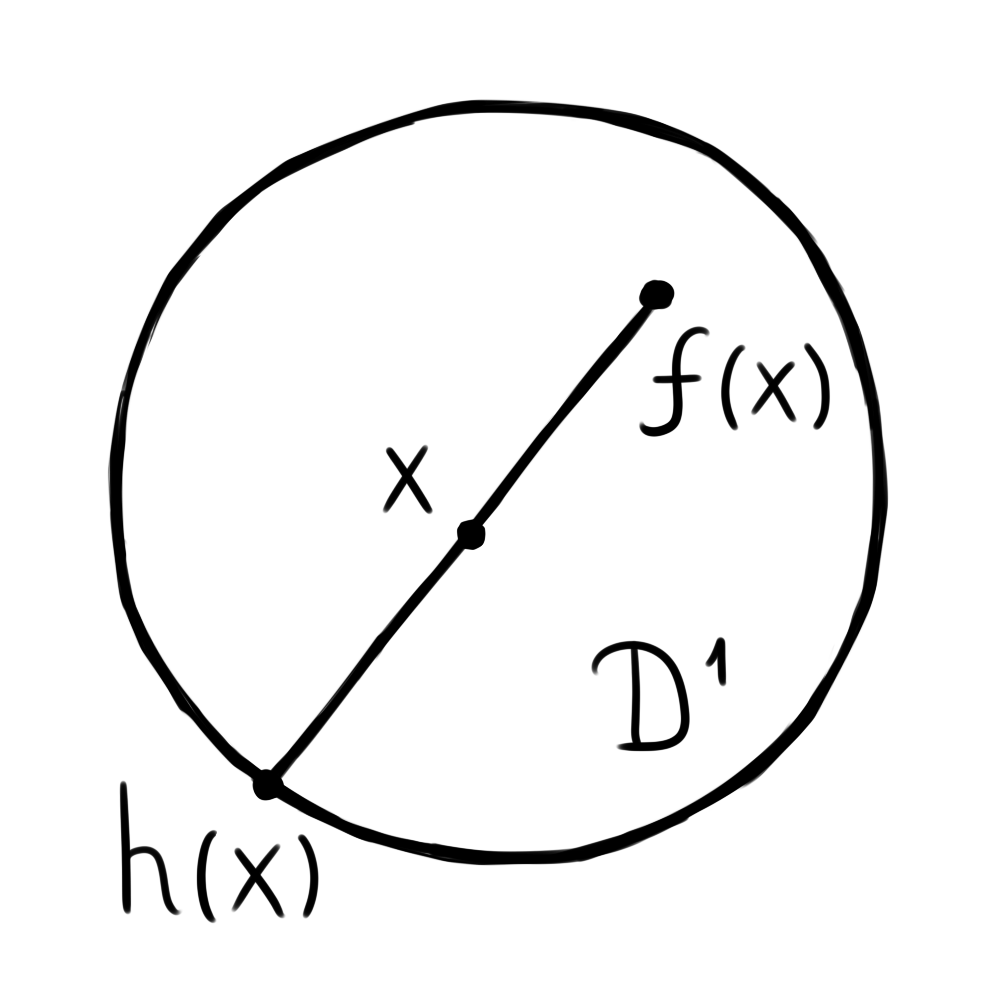
\includegraphics[width=0.5\textwidth]{brouwer}
	\end{figure}

	Определим отображение $ H \colon \S^1 \times [0;1] \to \S^1 $ следующим образом: для $ \vec{t} \in \S^1 $ и
	$ \tau \in [0;1] $ положим $ H(\vec{t}, \tau) = h(\tau \vec{t}) $. Оно непрерывно как композиция непрерывных
	отображений. Заметим, для любого $ \vec{t} \in \S^1 $ верно $ h_0(\vec{t}) = h(0) $:
	мы имеем константу. Значит, $ \Ind(h_0) = 0 $. Но $ h_1(\vec{t}) = h(\vec{t}) = \vec{t} $, откуда
	$ \Ind(h_1) = 1 $. Но в силу непрерывности отображения $ H $ является гомотопией между $ h_0 $ и $ h_1 $, чего
	не может быть, так как они имют разные индексы. Противоречие.
\end{proof}

\begin{theorem}
	Пусть $ T $, $ T_1 $, $ T_2 $ --- топологические пространства, причем $ T = T_1 \times T_2 $.
	Тогда $ \pi_1(T) \simeq \pi_1(T_1) \oplus \pi_2(T_2) $.
\end{theorem}

\begin{corollary}
	$ \pi_1(\T) \simeq \Z^2 $.
\end{corollary}

\begin{remark}
	Подразумевается, что выбрана некоторая точка $ t = (t_1, t_2) \in T $ и фундаментальные группы рассматриваются
	относительно $ t $, $ t_1 $ и $ t_2 $ соответственно.
\end{remark}

\begin{proof}
	Рассмотрим отрбражение $ G \colon \pi_1(T_1) \oplus \pi_2(T_2) \to \pi_1(T) $, определенное следующим образом:
	для петель $ \phi_1 $ и $ \phi_2 $ выполнено $ G([\phi_1] \oplus [\phi_2]) = [(\phi_1, \phi_2)] $.

	Докажем, что оно корректно определено. Ясно, что $ \phi_1 \sim \phi_1' $, $ \phi_2 \sim \phi_2' $ $ \iaoi $
	$ [\phi_1] \oplus [\phi_2] = [\phi_1'] \oplus [\phi_2'] $. Надо доказать, что
	$ (\phi_1, \phi_2) \sim (\phi_1', \phi_2') $. Рассмотрим отображение $ F = (F_1, F_2) $, где $ F_1 $ --- гомотопия
	между $ \phi_1 $ и $ \phi_1' $, а $ F_2 $ --- гомотопия между $ \phi_2 $ и $ \phi_2' $. Тогда отображение $ F $
	непрерывно как пара непрерывных отображений, а значит, является гомотопией между $ (\phi_1, \phi_2) $ и
	$ (\phi_1', \phi_2') $.

	Аналогично рассматривается отображение $ G^{-1} \colon \pi_1(T) \to \pi_1(T_1) \oplus \pi_2(T_2) $, обратное к
	отображению $ G $. Остается доказать только гомоморфность:
	\begin{multline*}
		G(([\phi_1] \oplus [\phi_2]) \cdot ([\phi_1'] \oplus [\phi_2']))
		= G([\phi_1 \phi_1'] \oplus [\phi_2 \phi_2'])
		= [(\phi_1 \phi_1', \phi_2 \phi_2')]
		= \\
		= [(\phi_1, \phi_2) \cdot (\phi_1', \phi_2')]
		= [(\phi_1, \phi_2)] \cdot [(\phi_1', \phi_2')]
		= G([\phi_1] \oplus [\phi_2]) \cdot G([\phi_1'] \oplus [\phi_2']).
	\end{multline*}
	Таким образом, $ G $ является изоморфизмом групп.
\end{proof}

Например, можно рассмотреть вид этого изоморфизма на торе. Пусть $ (a, b) \in \Z^2 $, тогда можно изобразить петлю
с <<индексом>> $ (a, b) $: она $ a $ раз проходит меридиан и $ b $ раз параллель.

\begin{figure}[H]
	\centering 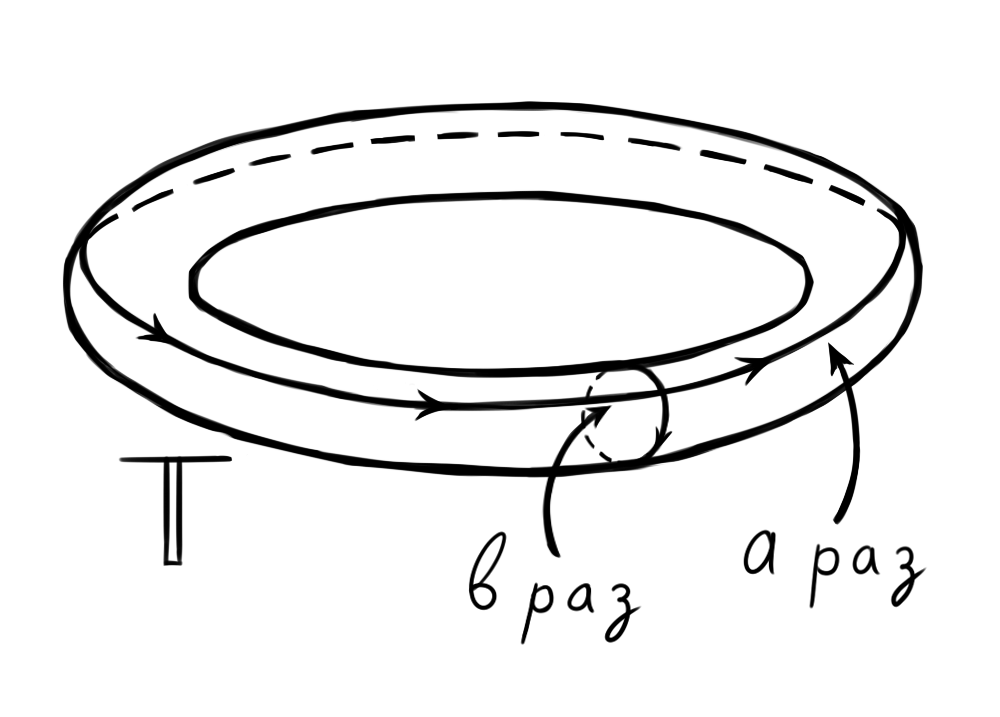
\includegraphics[width=0.5\textwidth]{torus-detour}
\end{figure}

\subsection{Гомотопическая эквивалентность топологических пространств}

Различные топологические пространства изучается путем анализа непрерывных отображений между ними. В качестве примера
рассмотрим задачу: при каких условия на топологические пространства $ T_1 $ и $ T_2 $ для любого топологического
пространства $ Z $ существует биекция между $ C(Z, T_1) $ и $ C(Z, T_2) $? Оказывается, достаточно гомеоморфности
$ T_1 \simeq T_2 $. Пусть $ f $ --- гомеоморфизм $ T_1 $ и $ T_2 $, тогда искомой биекцией будет отображение
$ f_* \colon g \mapsto f \circ g $, где $ g \in C(Z, T_1) $. Это биекция, так как для него существует
обратное отображение $ f_*^{-1} \colon h \mapsto f^{-1} \circ h $, где $ h \in C(Z, T_2) $. Но можно ли потребовать
чего-то меньшего, чем гомеоморфность?

Ближайшей целью будет определить понятие эквивалентности топологических пространств так, чтобы из эквивалентности
вытекала попарная эквивалентность гомотопических типов $ \pi(Z, T_1) $, $ \pi(Z, T_2) $ и $ \pi(T_1, Z) $,
$ \pi(T_2, Z) $ для любого топологического пространства $ Z $.

Раньше использовали гомеоморфизм $ f \colon T_1 \to T_2 $; как известно, для него существует такое отображение
$ g \colon T_2 \to T_1 $, что  $ g \circ f = \Id_{T_1} $ и $ f \circ g = \Id_{T_2} $. Но так как мы работаем с
множествами классов гомотопности, то нужно использовать гомотопность отображений: сопоставим классу
$ [h] \in \pi(Z, T_1) $ класс $ f_*([h]) \in \pi(Z, T_2) $ так, чтобы было верно $ (g_* \circ f_*) ([h]) = [h] $.
Таким образом, если раньше мы требовали полное равенство, то сейчас требуем только
$ g \circ f \circ h \sim h $. Оказывается, для того, чтобы этого добиться, достаточно лишь двух условий:
$ g \circ f \sim \Id_{T_1} $ и $ f \circ g \sim \Id_{T_2} $. Таким образом, вместо гомеоморфности получили
более слабое условие. Введем теперь это формально.

\begin{definition}
	Топологические пространства $ T_1 $ и $ T_2 $ называются \emph{гомотопически эквивалентными}, если существуют такие
	отображения $ f \colon T_1 \to T_2 $ и $ g \colon T_2 \to T_1 $, что $ g \circ f \sim \Id_{T_1} $ и
	$ f \circ g \sim \Id_{T_2} $; в этом случае пишут $ T_1 \sim T_2 $.
\end{definition}

\begin{restatable}{exercise}{ExcXV}
	Пусть $ A \ssq \R^n $ --- выпуклое множество, тогда $ A \sim \pt $.
\end{restatable}

\end{document}
